%!TEX root = ../thesis.tex

\section{Programación Funcional Reactiva}  %Title of the First Chapter

\ifpdf
    \graphicspath{{FRP/Figs/Raster/}{FRP/Figs/PDF/}{FRP/Figs/}}
\else
    \graphicspath{{FRP/Figs/Vector/}{FRP/Figs/}}
\fi

La programación reactiva funcional (FRP, por sus siglas en inglés) es un enfoque elegante para especificar de forma declarativa los sistemas reactivos, que son sistemas orientados en la propagación de cambios de múltiples entidades.

FRP integra la idea de flujo de tiempo y composición de eventos en la programación puramente funcional. Al manejar el flujo de tiempo de manera uniforme y generalizada, una aplicación obtiene claridad y fiabilidad. Así como la evaluación perezosa puede eliminar la necesidad de estructuras de control complejas, una noción uniforme de flujo de tiempo soporta un estilo de programación más declarativo que oculta un complejo mecanismo subyacente. Esto proporciona una manera elegante de expresar la computación en dominios como animaciones interactivas \cite{eh97:fran}, robótica \cite{Pembeci:2002:FRR:571157.571174}, visión por computadora, interfaces de usuario \cite{czaplicki2012elm} y simulación.

Las implementaciones más comunes de FRP para haskell  hacen uso de la notación de flechas, que son una nueva manera abstracta de visualizar los cómputos, creada por John Hughes \cite{hughes2000generalising}. Las flechas, al igual que los monads, proveen una estructura común para la implementación de librerías siendo más generales que los monads. John Hughes demostró que existen tipos de datos que no se adaptan bien a la estructura de monads causando así fugas de memoria indeseadas, que con flechas pueden ser resueltas en lenguajes funciones como haskell \cite{hughes2000generalising}. Adicionalmente las librerías de FRP en haskell usan una extensión del lenguaje propuesta por Ross  Paterson \cite{paterson2001new} que hace el uso de flechas mucho más fácil y conveniente que la versión original creada por Hughes. Para más detalles de la evolución de FRP leer ``Elm: Concurrent FRP for Functional GUIs'' \cite{czaplicki2012elm} capítulo 2.1.

En su más simple forma, FRP tiene dos abstracciones principales: Comportamientos, que cambian continuamente y Eventos que suceden en diferentes puntos en el tiempo. La continuidad del tiempo hace que estas abstracciones se puedan componer.

\section{Yampa}

Yampa es un lenguaje embebido para la programación de sistemas híbridos (tiempo discreto y continuo) utilizando los conceptos de Programación Reactiva Funcional (FRP). Yampa está estructurado con flechas, que reducen en gran medida la posibilidad de introducir fugas de espacio y tiempo en sistemas reactivos que varían en el tiempo \cite{wiki:Yampa}. Yampa es un sistema diseñado en base a una noción de muestreo y cambios dirigidos por eventos, es decir, la generación de un evento (como el presionar una tecla) causa la evaluación de valores y cambios en el estado actual del programa.

\subsection{Señales.}
En FRP una señal puede representar cualquier valor mutable. Estas pueden ser transformadas y combinadas, que a diferencia de otras soluciones más tradiciones, permite abstraer varios detalles menores, permitiendo al programador lograr un mismo resultado usando menos código. En Yampa una señal es una función que retorna un valor según el tiempo transcurrido, dicho en otras palabras, es una función que dado un tiempo determinado regresa el valor adecuado para el objeto mutable en el momento indicado. Un ejemplo es la posición del ratón.

\begin{equation}
Signal \ \alpha \approx Time \rightarrow \alpha
\end{equation}

\subsection{Funciones de señal.}
Es una función que recibe una señal y produce otra señal. Estas funciones permiten alterar o generar nuevas señales dependiendo del estado actual de la señal original, por ejemplo, puede ser deseable generar una señal nueva cuando el ratón pasa por sobre algún elemento gráfico en específico.

\begin{equation}
SF \ \alpha \ \beta \approx Signal \ \alpha \rightarrow Signal \ \beta
\end{equation}

Las funciones de señal son evaluadas de forma discreta a medida pasa el tiempo, al ser evaluadas retornan su valor de trabajo actual. Las SF pueden ser vistas como el comportamiento de un objeto, que cambia a medida que transcurre el tiempo.

\subsection{Combinadores de funciones de señal.}

Similar a la composición de funciones, las SF pueden ser compuestas para permitir un mejor filtrado de las señales. En Yampa los combinadores básicos son:

\begin{itemize}
\item arr: crea un SF a partir de una función Figura~\ref{fig:Yampa-arr}.
\item first: aplica una SF solo al primer elemento de la entrada y deja el resto sin cambios Figura~\ref{fig:Yampa-first}.
\item composición: compone dos SF, la señal resultada de la primera SF es dada como entrada a la segunda SF Figura~\ref{fig:Yampa-composition}.
\item loop: crea una SF que usa su propia salida para calcular su salida, que es posible gracias a la evaluación perezosa de los lenguajes funciones Figura~\ref{fig:Yampa-loop}.
\end{itemize}


\begin{figure}[htbp!]
\centering
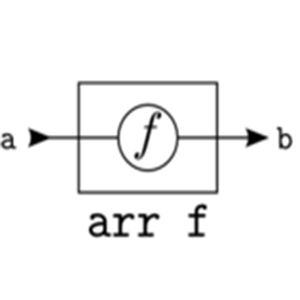
\includegraphics[width=0.4\textwidth]{Yampa-arr}
\caption[Yampa-arr]{Torna una función en SF.}
\label{fig:Yampa-arr}
\end{figure}

\begin{figure}[htbp!]
\centering
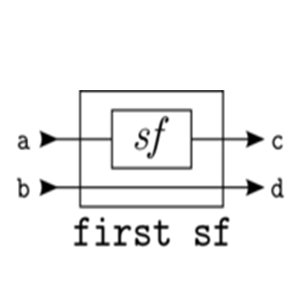
\includegraphics[width=0.4\textwidth]{Yampa-first}
\caption[Yampa-first]{Aplica un SF al primer elemento.}
\label{fig:Yampa-first}
\end{figure}

\begin{figure}[htbp!]
\centering
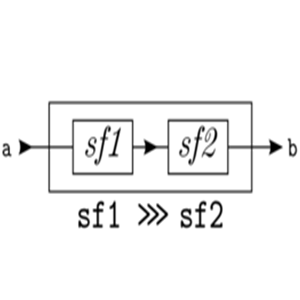
\includegraphics[width=0.4\textwidth]{Yampa-composition}
\caption[Yampa-composition]{Compone dos SF.}
\label{fig:Yampa-composition}
\end{figure}

\begin{figure}[htbp!]
\centering
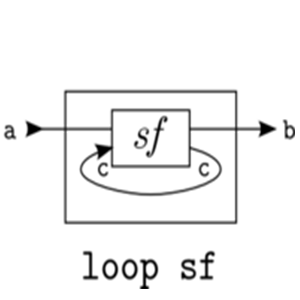
\includegraphics[width=0.4\textwidth]{Yampa-loop}
\caption[Yampa-loop]{Yampa loop}
\label{fig:Yampa-loop}
\end{figure}

Partiendo de estos combinadores se pueden derivar todos los combinadores más complejos usados por la librería Yampa.

\subsection{Interruptores}

Los interruptores (Figura~\ref{fig:Yampa-switch}) son elementos que permiten que las SF sean comportamientos capaces de cambiar en base a eventos externos además de cambiar con el tiempo. Los interruptores dan a las SF propiedades similares a la de una máquina de estados, donde los eventos causan una transición de un comportamiento a otro.

\begin{figure}[htbp!]
\centering
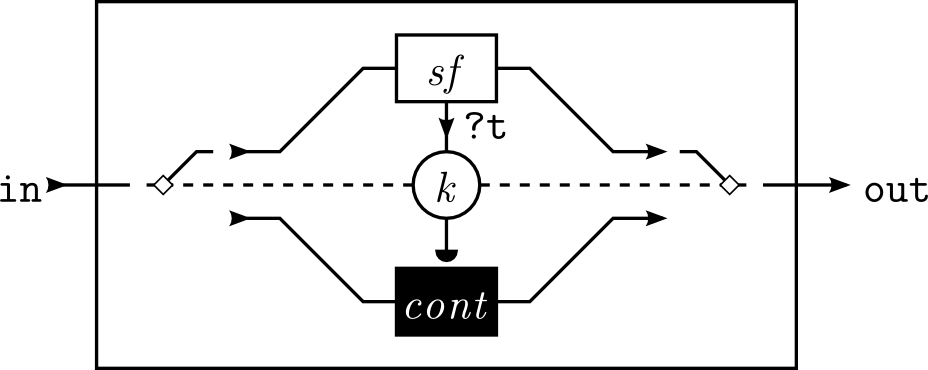
\includegraphics[width=0.4\textwidth]{Yampa-switch}
\caption[Yampa-switch]{Una SF cambia a una continuación al dispararse una condición k.}
\label{fig:Yampa-switch}
\end{figure}

\subsection{Usando Yampa}

Las funciones de señal se pueden crear y manipular a través de la interfaz de Arrow. Por ejemplo, una transformación pura (a -> b) se convierte en una función de señal simplemente con arr de la clase Arrow. Aquí hay una función de señal que eleva a dos los valores que pasan a través de ella:

\begin{lstlisting}[frame=single]
square :: SF Double Double
square = arr (^2)
\end{lstlisting}

La función de utilidad \textbf{embed}  se puede usar para probar funciones de señal:

\begin{lstlisting}[frame=single]
embed square (1, [(0, Just 2), (1, Just 3)])
[1.0,4.0,9.0]
\end{lstlisting}

La firma de la función \textbf{embed} se ve así:

\begin{lstlisting}[frame=single]
embed :: SF a b -> (a, [(DTime, Maybe a)]) -> [b]
\end{lstlisting}

El primer argumento es la función de señal a muestrear. El segundo es una tupla que consiste en la entrada inicial a la función de señal y una lista de tiempos de muestra, posiblemente acompañada de un nuevo valor de entrada.

Un evento que contiene un valor de tipo a está representado por el Evento a:

\begin{lstlisting}[frame=single]
data Event a = Event a | NoEvent
\end{lstlisting}

Una fuente de evento es una función de señal con algún tipo SF a (Evento b). Algunos ejemplos de fuentes de eventos son los siguientes:

\begin{lstlisting}[frame=single]
never :: SF a (Event b)
now :: b -> SF a (Event b)
after :: Time -> b -> SF a (Event b)
\end{lstlisting}

Como el origen del evento es solo un SF normal, podríamos generar eventos con arr. Sin embargo, entonces debemos tener cuidado de que el evento se emita solo una vez: debido a que las uniones de señal son continuas, a menos que el evento se suprima en muestreos posteriores, podría ocurrir más de una vez.

Para reaccionar en eventos, necesitamos interruptores. El interruptor básico de una sola vez tiene el siguiente tipo:

\begin{lstlisting}[frame=single]
switch :: SF a (b, Event c) -- SF por defecto
          -> (c -> SF a b)   -- SF despues del evento
          -> SF a b
\end{lstlisting}

La siguiente señal produce la cadena foo durante los primeros 2 segundos, después de lo cual se dispara un evento y se produce bar:

\begin{lstlisting}[frame=single]
switchFooBar, switchFooBar' :: SF () String
switchFooBar = switch (constant "foo"&&& after 2 "bar") constant
switchFooBar' = dSwitch (constant "foo"&&& after 2 "bar") constant
\end{lstlisting}

La función dSwitch es idéntica a switch, excepto que, en el momento del evento, en la segunda el cambio es inmediato, en la primera el cambio se genera al siguiente muestreo.

\begin{lstlisting}[frame=single]
> embed switchFooBar ((), [(2, Nothing), (3, Nothing)])
["foo","bar","bar"]
> embed switchFooBar' ((), [(2, Nothing), (3, Nothing)])
["foo","foo","bar"]
\end{lstlisting}

Ejemplos mostrados en esta sección fueron creados por Samuli Thomasson, si el lector quiere profundizar en el uso de Yampa leer ``Haskell High Performance Programming'' \cite{thomasson2016haskell} capítulo 13.
